% ju 28-Mai-22
\documentclass[a4paper,12pt,fleqn,parskip=half]{scrartcl}
\usepackage[ngerman]{babel}
\usepackage[utf8]{inputenc}
\usepackage[T1]{fontenc}

% Schrift
%\usepackage{lmodern}
\usepackage[osf,sc]{mathpazo} 
\usepackage[scale=.9,semibold]{sourcecodepro}   
\usepackage[osf]{sourcesanspro}  

\usepackage[headsepline]{scrlayer-scrpage}
\pagestyle{scrheadings}
\clearpairofpagestyles

\usepackage[table,dvipsnames,usenames]{xcolor}
\usepackage{textcase}
\usepackage{nameref}
\usepackage{hyperref}
\usepackage{tabularx}
\usepackage{multirow}
\usepackage{multicol}
\usepackage{caption, booktabs}
\usepackage{graphicx} 
\usepackage{scrhack}    
\usepackage{url}%% Links
\usepackage[inline]{enumitem}
\usepackage{pifont}
\usepackage{eurosym}% \euro 20,-
\usepackage{amsmath}
\usepackage{amsfonts}
\usepackage{amssymb}
\usepackage{array}            % Extending the array and tabular environments
\usepackage{chngcntr}         % Change the resetting of counters
\usepackage[version=4]{mhchem}
\usepackage{stmaryrd}
\usepackage{siunitx}
\usepackage{float}
\usepackage{csquotes}
\usepackage{subcaption}
\usepackage{mathtools}
\usepackage{icomma}%Dezimaltrennzeichen
\usepackage{multimedia}%Video: \movie[externalviewer]{(video.mov)}{video.mov}
\usepackage{epstopdf}
\usepackage{footnote}
\usepackage{qrcode}% Anwendung: \qrcode[hyperlink,level=Q,version=2,height=1cm]{\website}
\usepackage{underscore}% Unterstrich ____

% PDF Dokumente einbinden
\usepackage{pdfpages}% \includepdf[pages=-]{Tabellen/Excel.pdf}
\RequirePackage{lastpage}  % Pagecounter

\addto\captionsngerman{%
\renewcommand{\figurename}{Abb.}
\renewcommand{\tablename}{Tab.}
}

% listings
\usepackage{listings}
\lstset{basicstyle=\linespread{1}\ttfamily\small,floatplacement=!htb,captionpos=t,abovecaptionskip=.5\baselineskip,belowcaptionskip=.5\baselineskip,upquote=true,showstringspaces=false,inputencoding=utf8,tabsize=4,
    	keywordstyle=\bfseries ,
	commentstyle=\color{rot5},
	stringstyle=\color{orange},
	breaklines=true,
  	postbreak=\mbox{\textcolor{black}{$\hookrightarrow$}\space},
	breakatwhitespace=false
}
\lstset{literate={á}{{\'a}}1 {é}{{\'e}}1 {í}{{\'i}}1 {ó}{{\'o}}1 {ú}{{\'u}}1 {Á}{{\'A}}1 {É}{{\'E}}1 {Í}{{\'I}}1 {Ó}{{\'O}}1 {Ú}{{\'U}}1 {à}{{\`a}}1 {è}{{\`e}}1 {ì}{{\`i}}1 {ò}{{\`o}}1 {ù}{{\`u}}1 {À}{{\`A}}1 {È}{{\'E}}1 {Ì}{{\`I}}1 {Ò}{{\`O}}1 {Ù}{{\`U}}1 {ä}{{\"a}}1 {ë}{{\"e}}1 {ï}{{\"i}}1 {ö}{{\"o}}1 {ü}{{\"u}}1 {Ä}{{\"A}}1 {Ë}{{\"E}}1 {Ï}{{\"I}}1 {Ö}{{\"O}}1 {Ü}{{\"U}}1 {â}{{\^a}}1 {ê}{{\^e}}1 {î}{{\^i}}1 {ô}{{\^o}}1 {û}{{\^u}}1 {Â}{{\^A}}1 {Ê}{{\^E}}1 {Î}{{\^I}}1 {Ô}{{\^O}}1 {Û}{{\^U}}1 {œ}{{\oe}}1 {Œ}{{\OE}}1 {æ}{{\ae}}1 {Æ}{{\AE}}1 {ß}{{\ss}}1 {ű}{{\H{u}}}1 {Ű}{{\H{U}}}1 {ő}{{\H{o}}}1 {Ő}{{\H{O}}}1 {ç}{{\c c}}1 {Ç}{{\c C}}1 {ø}{{\o}}1 {å}{{\r a}}1 {Å}{{\r A}}1 {€}{{\EUR}}1 {£}{{\pounds}}1 {~}{{\textasciitilde}}1 {-}{{-}}1 }

% bibliography
\usepackage[
    bibencoding=utf8,
    backend=biber,% bibtex, biber
    backref=false,backrefstyle=three+,url=true,urldate=comp,abbreviate=false,maxnames=20
]{biblatex} %Paket laden
\DeclareBibliographyCategory{cited}
\let\defaultcite\cite\renewcommand*\cite[2][]{\addtocategory{cited}{#2}\defaultcite[#1]{#2}}
\let\defaulttextcite\textcite\renewcommand*\textcite[2][]{\addtocategory{cited}{#2}\defaulttextcite[#1]{#2}}
\setcounter{biburllcpenalty}{7000}
\setcounter{biburlucpenalty}{8000}
\AfterPackage{biblatex}{
	\PreventPackageFromLoading[\errmessage{Sie haben versucht, das Cite-Paket zu laden, das nicht mit biblatex kompatibel ist.}]{cite}
}

\hypersetup{%
	%pdftitle={\titel},
	%pdfsubject={Latex},
	%pdfauthor={\autor},
	%pdfcreator={\autor}, 
	bookmarksnumbered=true,
	breaklinks=true,
	%colorlinks=true,	   
	linkcolor=rot5,		
	filecolor=blau5,		
	urlcolor=blau5,			
	citecolor=ForestGreen
}

\linespread{1.1}
\setlist{itemsep=0pt}
\widowpenalty10000
\clubpenalty10000
\tolerance1000   

\usepackage[left=2cm,right=2cm,top=1cm,bottom=1cm,includeheadfoot]{geometry}
%\usepackage[left=4cm,right=2cm,top=1cm, bottom=1cm,includeheadfoot]{geometry}
%\usepackage[left=6cm,right=1cm,top=1cm, bottom=1cm,includeheadfoot]{geometry}
%\usepackage[landscape=true,left=2cm,right=2cm,top=1cm,bottom=1cm,includeheadfoot]{geometry}%quer

% eigene Farbe definieren
% Adobe Prozessfarben: CMYK: 100,50,0,35 -> 1,0.5,0,0.35
\definecolor{orange}{cmyk}{0,0.55,0.61,0}   % 0,55,61,0
\definecolor{blau5}{cmyk}{1,0.77,0.1,0.01}  % 100,77,10,
\definecolor{rot5}{cmyk}{0.22,1,1,0.19}     % 22,100,100,19
\definecolor{grau2}{cmyk}{0,0,0,0.1}        % 0,0,0,40
\definecolor{blau}{cmyk}{0.93,0.66,0,0.21}% 

% Literatur
\bibliography{content/literatur}
\bibliography{content/literatur-kfz}
\bibliography{content/literatur-sport}

%%%%%%%%%%%%%%%%%%%%%%%%%%%%%%%%%%%%%%%%%%%%%%%%%%%%%%%
\newcommand{\name}{Jan Unger}% anpassen!!!!!
\newcommand{\thema}{03-Grundlagen-Elektrik2}
\newcommand{\quelle}{\name}
\newcommand{\website}{https://bw-ju.de/}
\newcommand{\github}{https://github.com/ju1-eu}
%%%%%%%%%%%%%%%%%%%%%%%%%%%%%%%%%%%%%%%%%%%%%%%%%%%%%%%

\ihead{\textbf{Quelle:} \quelle}%{Kopfzeile innen}
\ohead{\textbf{Datum:} \today}  %{Kopfzeile außen}

\ifoot{\textbf{Thema:} \thema}  %{Fußzeile  innen}
\ofoot{Seite {\thepage} von {\pageref{LastPage}}}%{Fußzeile  außen}

\title{\thema}
\author{\name}
\date{\today}

\begin{document}
	%\thispagestyle{empty}
	%\maketitle
	%\newpage
	%\setcounter{page}{1}

	%%%%%%%%%%%%%%%%%%%%%%%%%%%%%%%%%%%%%%%%%%%
	\begin{center}
		\textbf{\Large \thema}%14pt
		\vspace{0.8em}
		
		%\datum	
		%\qrcode[hyperlink,level=Q,version=2,height=1cm]{\website}
		\qrcode[hyperlink,level=Q,version=2,height=1cm]{\github}
	\end{center}
	%%%%%%%%%%%%%%%%%%%%%%%%%%%%%%%%%%%%%%%%%%%

	\subsection*{Keywords}%\label{sec:Deadline}\index{Deadline}
	% Checkliste
	\begin{itemize}[label=\checkmark] %\itemsep -2pt
		\item Begriff 
	\end{itemize}

    %%%%%%%%%%%%%%%%%%%%%%%%%%%%%%%%%%%%%%%%%%%%%%%%%%%%%%%%%%%%%%%%%%

	% anpassen
	%\input{content/tex/neu}
	%ju 28-Mai-22 03-Grundlagen-Elektrik2.tex
\section{Potentialbestimmung}\label{potentialbestimmung}

\begin{figure}[!ht]% hier: !ht
\centering
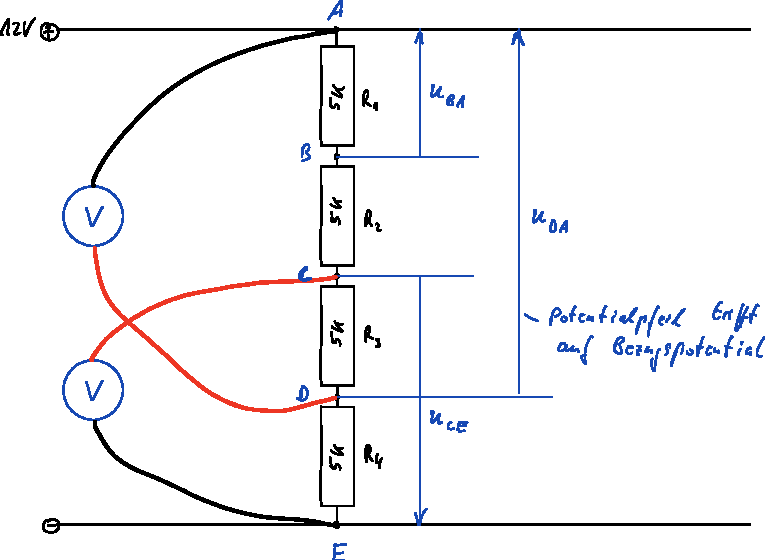
\includegraphics[width=0.6\textwidth]{images/Skizze/28_FT_Potentialbestimmung.pdf}
\caption{Potentialbestimmung}
%\label{fig:}%% anpassen
\end{figure}

Klemmenspannung und Potential

\begin{itemize}
\item
  $U_{R_1} = 3~V$, $U_{R_3} = 3~V$
\item
  $U_{CE} = 6~V$, $U_{BA} = -3~V$, $U_{DA} = -9~V$
\end{itemize}

Möchte man das/ein Potential an einem Punkt in einem Stromkreis
messen/bestimmen, bezieht man sich immer auf ein Bezugspotenzial. Die
Schreibweise dieser Messung lautet dann zum Beispiel $U_{CE}$, hierbei
möchte ich also das Potential C messen, C ist der erste Buchstabe, an
ihm wird der \emph{rote Clip} des Multimeters angeschlossen. Das
Bezugspotenzial hierbei E ist der zweite Buchstabe, hier wird
grundsätzlich der \emph{schwarze Clip} des Multimeters angeschlossen.
Potentialbestimmungen können auch zeichnerisch dargestellt werden.
Hierbei lautet die Vereinbarung, die Pfeilspitze des Spannungs- oder
Potentialpfeils trifft immer auf das Bezugspotenzial. Beispiel
$U_{DA}$.

\newpage

\section{Brückenschaltung -
Brückenspannung}\label{brueckenschaltung-brueckenspannung}

\begin{figure}[!ht]% hier: !ht
\centering
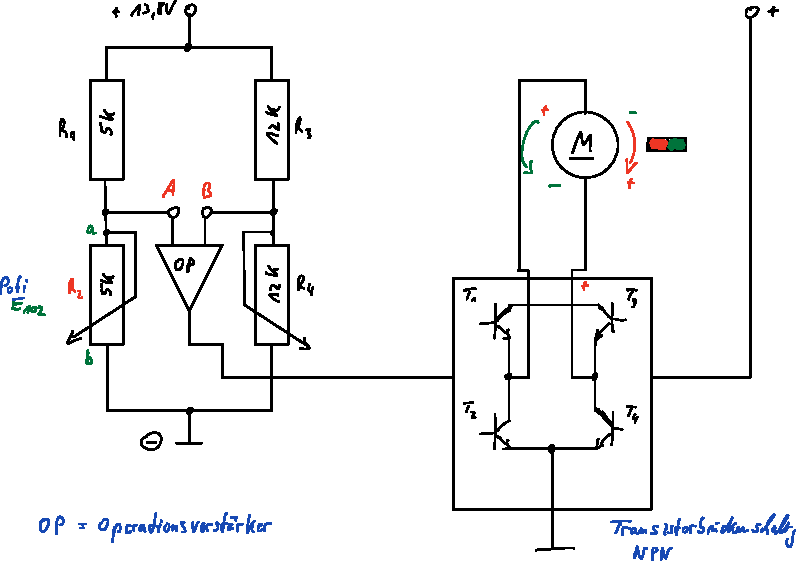
\includegraphics[width=0.6\textwidth]{images/Skizze/28_FT_Brueckenschaltung.pdf}
\caption{Brückenschaltung}
%\label{fig:}%% anpassen
\end{figure}

$U_{A\text{-}} = 6,9~V$, $U_{B\text{-}} = 6,9~V$, $U_{AB} = 0~V$
(keine Differenz)

$U_{A\text{+}} = -6,9~V$, $U_{B\text{+}} = -6,9~V$, $U_{AB} = 0~V$
(keine Differenz)

Poti $\to R_2 = 1~k$

$I_{Li} = \frac{U_{ges}}{R_{{Li}_{ges}}} = \frac{U_{ges}}{R_1 + R_2} = \frac{13,8}{5000 + 1000} =0,0023~A$

$U_{R_1} = R_1 \cdot I_{Li} = 5000~\Omega \cdot 0,0023~A = 11,5~V$

$U_{A\text{+}} = -11,5~V$, $U_{B\text{+}} = -6,9~V$,
$U_{AB} = -4,6~V$

$I_{Re} = \frac{U_{R_3}}{R_3} = \frac{11,5}{12000} =0,00096~A$

$R_4 = \frac{U_{R_4}}{I_{Re}} = \frac{U_{ges} - U_{R_3}}{I_{Re}} = \frac{13,8 - 11,5}{0,00096} = 2395,83~\Omega$

\newpage

\section{Signalanlage Oldtimer
(Prüfung)}\label{signalanlage-oldtimer-pruefung}

\textbf{Aufgabe:} Stromlaufplan zeichnen

Ein Kunde beanstandet Folgendes:

\textbf{>>Wenn ich den Fahrtrichtungsanzeiger setze und dabei das
Bremspedal betätige, bleibt mein Fahrtrichtungsanzeiger stehen.<<}

Lösen Sie dieses Problem mit einem entsprechenden Relaisschaltung.
Komponenten, die vorhanden sein müssen: Batterie, 30/15/31ger Schiene,
Blinkrelais (2-polig), Kontrollleuchte, Blinkerschalter, zwei
Blinkleuchten links, zwei Blinkleuchten rechts. Dazu ein entsprechendes
Relais.

\textbf{Problem - Spannungsverlust durch Bremse treten}

\begin{figure}[!ht]% hier: !ht
\centering
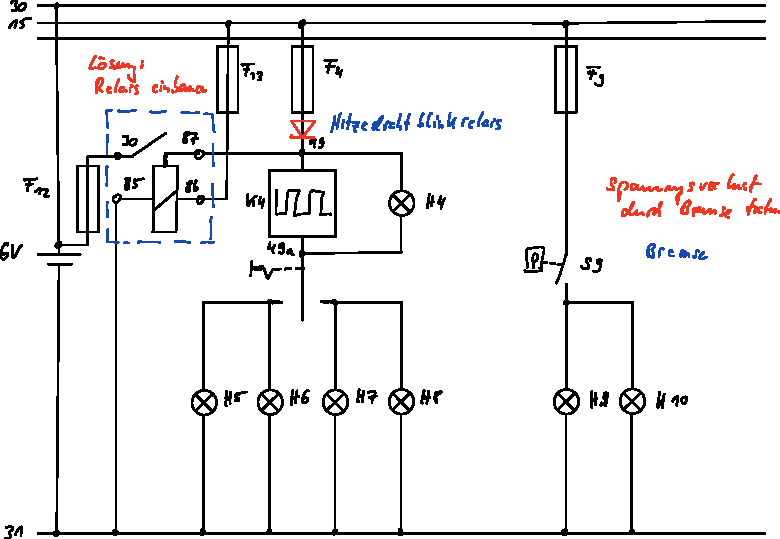
\includegraphics[width=0.9\textwidth]{images/Skizze/29_FT_Signalanlage_Relais_6V.pdf}
\caption{Signalanlage Oldtimer Relais}
%\label{fig:}%% anpassen
\end{figure}

\emph{Lösung} $\to$ Relais einbauen.

\emph{Zündung Einschalten} Steuerstrom baut magnetisches Feld auf und
schneidet die Spule, induziert dabei eine Spannung von $6~V$.

\textbf{Blinkfrequenz} $90 \pm30$ Impulse pro Minute

\emph{Zündung ausschalten} Diode einbauen zwischen F4 und Anschluß 49

\newpage

\section{Tagfahrlicht verdrahten mit Relais Öffner oder
Schließer}\label{tagfahrlicht-verdrahten-mit-relais-oeffner-oder-schliesser}

\textbf{Vorteile LED}

\begin{itemize}
\item
  Stromverbrauch
\item
  Haltbarkeit
\item
  Bezeichnung >>RL<<
\item
  Abstand $600~mm$
\end{itemize}

\begin{figure}[!ht]% hier: !ht
\centering
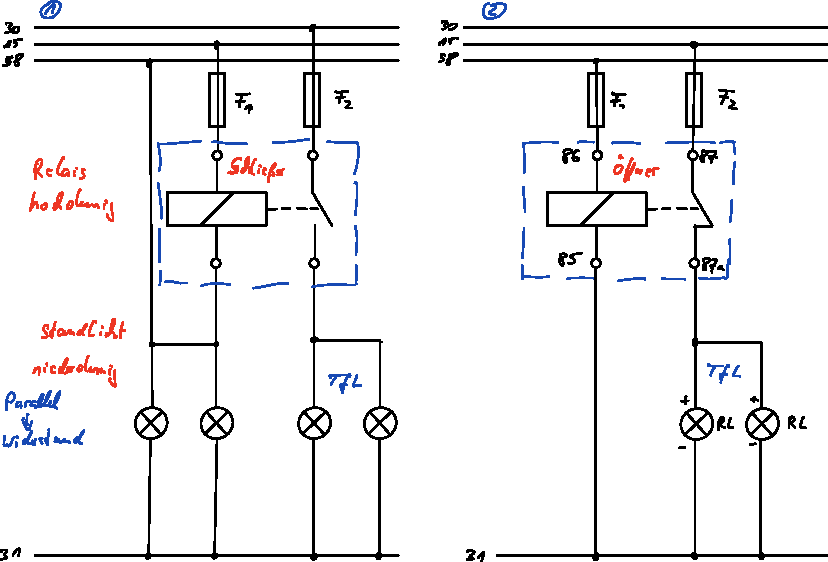
\includegraphics[width=0.9\textwidth]{images/Skizze/29_FT_Tagfahrlicht_Relais.pdf}
\caption{Tagfahrlicht Relais}
%\label{fig:}%% anpassen
\end{figure}

\textbf{1) Wieso leuchtet das Tagfahrlicht ohne Standlicht?} - Das
Relais ist hochohmig und das Standlicht (4x Lampen parallel) ist
niederohmig. - Das Relais holt sich die Masse über die Lampen.

\textbf{2) Was muss ich machen, damit ich Kraftstoff einsparen kann?} -
Vgl. Abb. Tagfahrlicht - (1) Sicherung \emph{F1} ziehen - (2) Sicherung
\emph{F1} und \emph{F2} ziehen

\newpage

\section{Elektromotorarten}\label{elektromotorarten}

\subsection{Nebenschlussmotor}\label{nebenschlussmotor}

Urmotor im Kfz, außer Starter

\begin{table}[!ht]% hier: !ht 
\centering 
	\caption{}% \label{tab:}%% anpassen 
\begin{tabular}{@{}ll@{}}
\hline
\textbf{Abk.} & \textbf{Bezeichnung} \\
\hline
$AW$ & Ankerwicklung (Spule) \\
$NSW$ & Nebenschlusswicklung (Spule) \\
$I_A$ & Ankerstrom \\
$I_{NSW}$ & Stromfluss durch die NSW \\
$RSW$ & Reihenschlusswicklung \\
$I_{RSW}$ & Stromfluss durch die RSW \\
\hline
\end{tabular} 
\end{table}

\textbf{a) Nebenschlussmotor mit Feldwicklung}

Kennlinie - Drehzahlverhalten

\begin{figure}[!ht]% hier: !ht
\centering
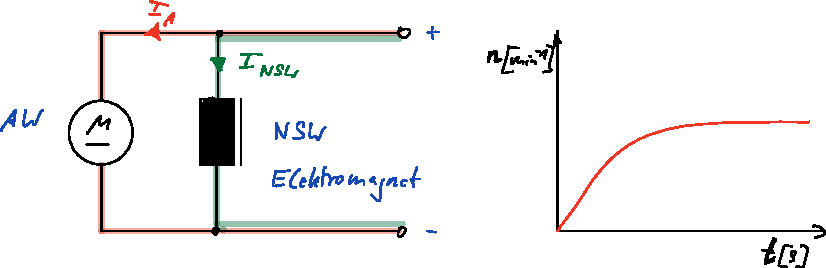
\includegraphics[width=0.6\textwidth]{images/Skizze/30_FT_Nebenschlussmotor_mit_Feldwicklung.pdf}
\caption{Nebenschlussmotor mit Feldwicklung}
%\label{fig:}%% anpassen
\end{figure}

\textbf{b) Nebenschlussmotor mit Permanenterregung}

Kennlinie - Drehzahlverhalten

\begin{figure}[!ht]% hier: !ht
\centering
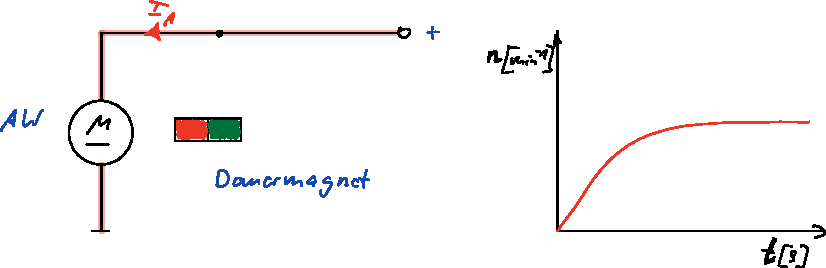
\includegraphics[width=0.6\textwidth]{images/Skizze/30_FT_Nebenschlussmotor_mit_Permanenterregung.pdf}
\caption{Nebenschlussmotor mit Permanenterregung}
%\label{fig:}%% anpassen
\end{figure}

\subsection{Reihenschlussmotor}\label{reihenschlussmotor}

Dreht hoch

Kennlinie - Drehzahlverhalten

\begin{figure}[!ht]% hier: !ht
\centering
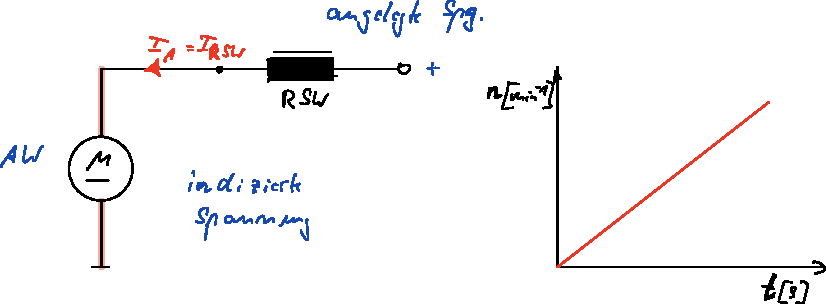
\includegraphics[width=0.6\textwidth]{images/Skizze/30_FT_Reihenschlussmotor.pdf}
\caption{Reihenschlussmotor}
%\label{fig:}%% anpassen
\end{figure}

\subsection{Doppelschlussmotor}\label{doppelschlussmotor}

Hohe Leistung

Kennlinie - Drehzahlverhalten

\begin{figure}[!ht]% hier: !ht
\centering
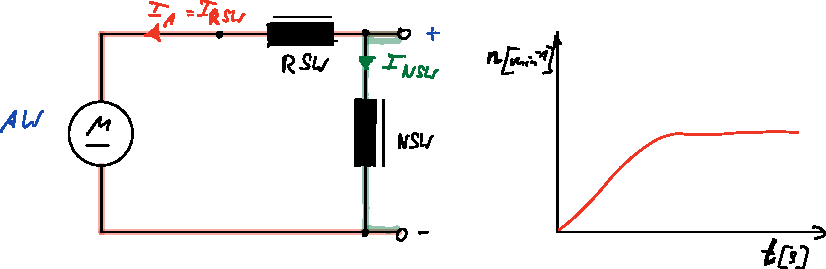
\includegraphics[width=0.6\textwidth]{images/Skizze/30_FT_Doppelschlussmotor.pdf}
\caption{Doppelschlussmotor}
%\label{fig:}%% anpassen
\end{figure}

\subsection{Wechselstrommotor}\label{wechselstrommotor}

Kennlinie - Drehzahlverhalten

\begin{figure}[!ht]% hier: !ht
\centering
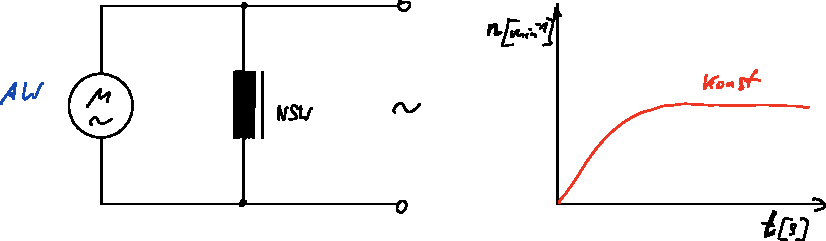
\includegraphics[width=0.6\textwidth]{images/Skizze/30_FT_Wechselstrommotor.pdf}
\caption{Wechselstrommotor}
%\label{fig:}%% anpassen
\end{figure}

\subsection{Schrittmotor}\label{schrittmotor}

Anwendung: Sitzverstellung, Scheinwerferhöhenverstellung, Schiebedach

Kennlinie - Drehzahlverhalten

\begin{figure}[!ht]% hier: !ht
\centering
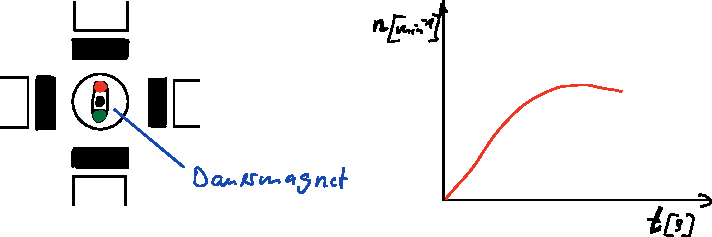
\includegraphics[width=0.6\textwidth]{images/Skizze/30_FT_Schrittmotor.pdf}
\caption{Schrittmotor}
%\label{fig:}%% anpassen
\end{figure}

\subsection{Drehstrommotor}\label{drehstrommotor}

Dozentenwechsel \ldots{}


	%%%%%%%%%%%%%%%%%%%%%%%%%%%%%%%%%%%%%%%%%%%%%%%%%%%%%%%%%%%%%%%%%%
    % Bibliographie
    \printbibliography
\end{document}
